\documentclass{beamer}
\usetheme{Boadilla}
\setbeamertemplate{navigation symbols}{}
\setbeamercovered{invisible}
\useinnertheme{rounded}

%Palatino + AMS Euler
\usepackage[euler-digits,euler-hat-accent]{eulervm}
\usefonttheme{serif}
\usepackage{fontspec}
%\setmainfont{TeX Gyre Pagella}


\usepackage{tikz}
\usepackage{tikzscale}
\usetikzlibrary{shapes,arrows.meta}
\usetikzlibrary{positioning}
\usetikzlibrary{math}
\usetikzlibrary{external}
\tikzexternalize[optimize=false,prefix=tikz/]
\usepackage{amssymb}
\usepackage{nicefrac}
\usepackage{amsmath}
\usepackage{siunitx}
\usepackage{mathtools}
\usepackage{booktabs}
\usepackage{graphicx}
\sisetup{range-phrase=~...~}
\usepackage{pgfgantt}
\usepackage{soul}
\usepackage{pgfplots}
\pgfplotsset{compat=newest}
\usepgfplotslibrary{fillbetween}
\usepgfplotslibrary{groupplots}
\usepackage{listings}
\usepackage{tabularx}
\usepackage{subfig}

\definecolor{juasblue}{rgb}{0,0.5411,0.7647}
\definecolor{juasgrey}{rgb}{0.49,0.698,0.761}
\graphicspath{ {./img/}}

\title[Practical Days - RF]{CERN practical days - RF}
\subtitle{09:00} 
\author[Heine, Noll]{Ruben Heine \and Marvin Noll}
\date[\today]{14.03.2022}

\makeatletter
\colorlet{beamer@blendedblue}{juasblue}
\makeatother

\begin{document}
\begin{frame}[plain]
  \titlepage
\end{frame}

\begin{frame}{Outline}
    \tableofcontents
\end{frame}

\section{Forenoon Session}
\subsection{Band Pass Filter}
\begin{frame}[t,fragile]{Band Pass Filter (1) - Transmission $S_{12}$, $S_{21}$}
\begin{figure}
  \centering
  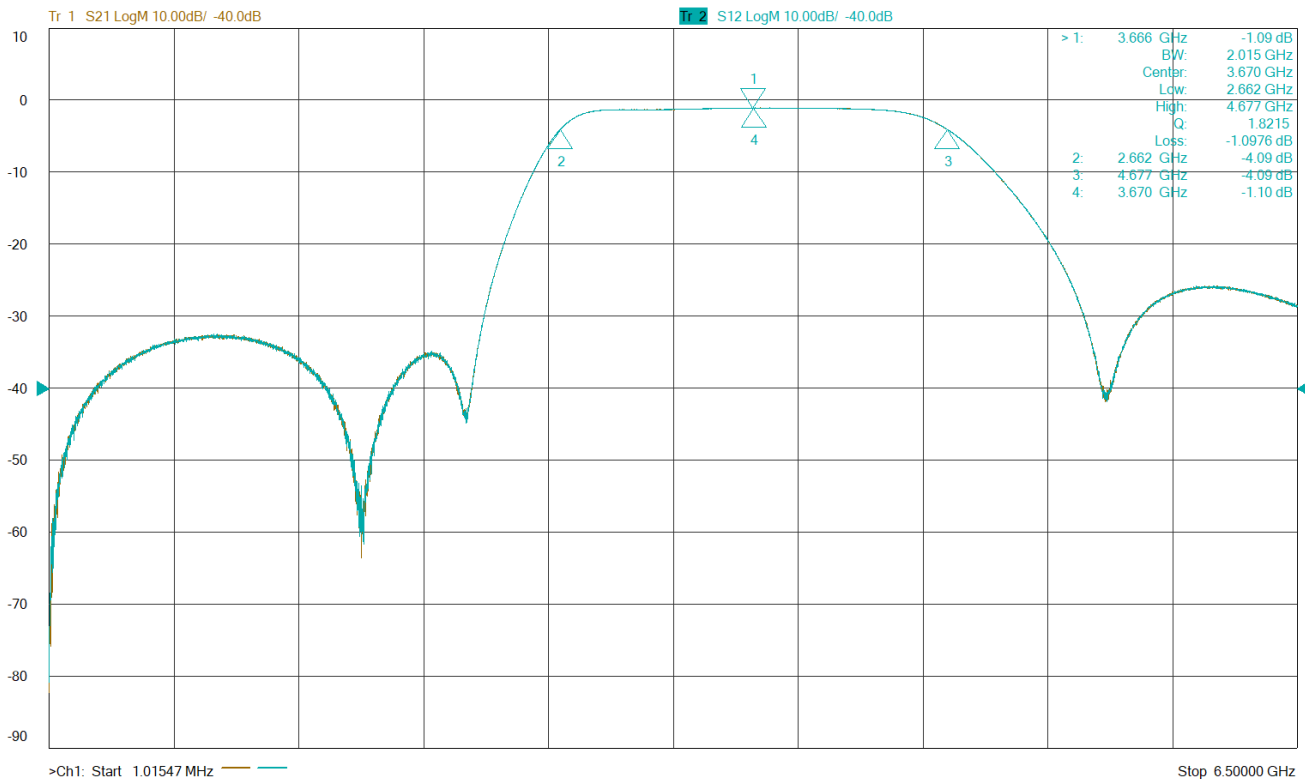
\includegraphics[width=0.9\textwidth]{img/bandpass_S12.png}
\end{figure}
\begin{equation*}
BW=\SI{2.015}{\GHz},\quad f=\SIrange{2.66}{4.67}{\GHz}
\end{equation*}
\begin{center}
$S_{21} \approx S_{12} \Rightarrow$ Reciprocal
\end{center}
\end{frame}

\begin{frame}[t,fragile]{Band Pass Filter (2) - Input/Output Reflection $S_{11}$, $S_{22}$}
\begin{figure}
  \centering
  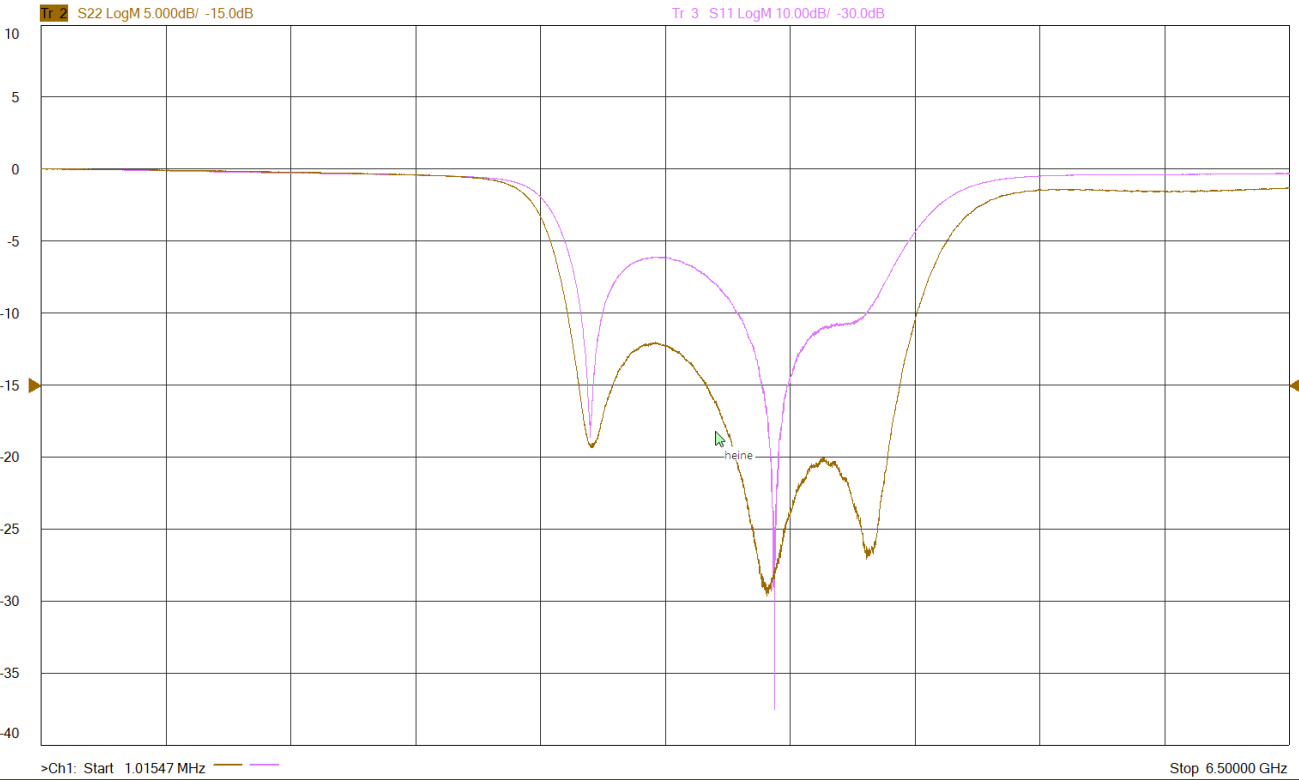
\includegraphics[width=0.9\textwidth]{img/bandpass_S11S22.png}
\end{figure}
\begin{center}
$S_{11} \neq S_{22} \Rightarrow$ Non symmetric
\end{center}
\end{frame}

\begin{frame}[t,fragile]{Band Pass Filter (3) - Phase $\angle S_{12}$}
\begin{figure}
  \centering
  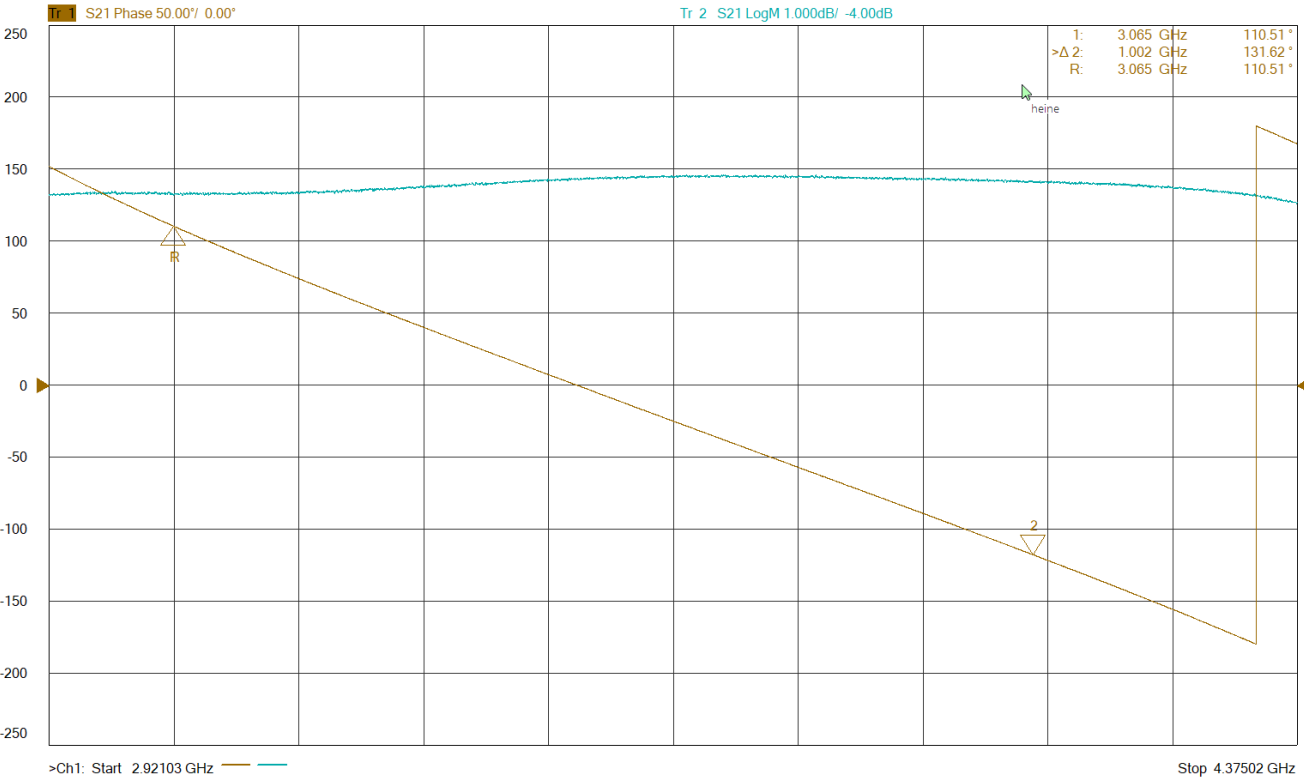
\includegraphics[width=0.9\textwidth]{img/bandpass_phase.png}
\end{figure}
\begin{equation*}
t_g = - \frac{\text{d}}{\text{d}\omega} \angle S_{12} \approx -\frac{\Delta \angle S_{12} \;[\si{\radian}]}{\Delta \omega} = \frac{\SI{2.297}{\radian}}{\SI{1.002}{\GHz}} = zu wenig
\end{equation*}
\end{frame}

\begin{frame}[t,fragile]{Band Pass Filter (3) - Group Delay $t_g$}
\begin{figure}
  \centering
  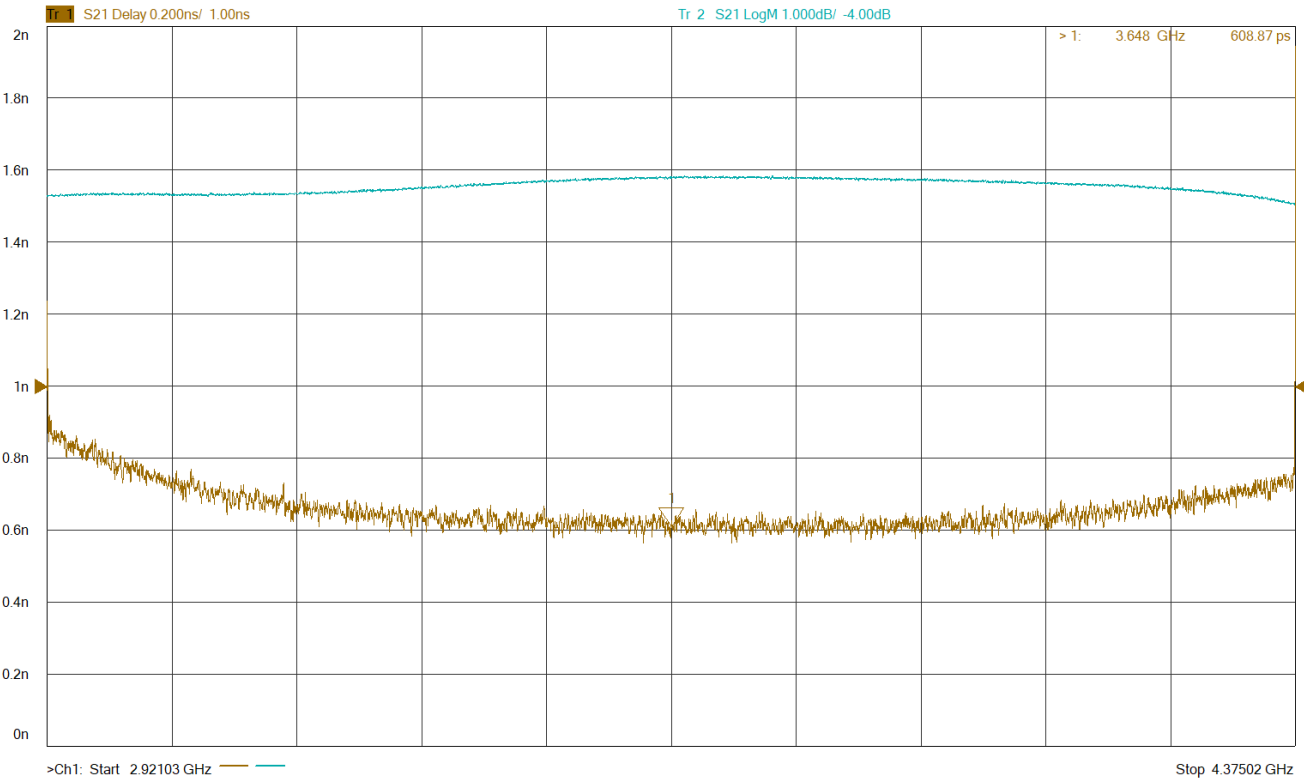
\includegraphics[width=0.9\textwidth]{img/bandpass_groupdelay.png}
\end{figure}
\begin{equation*}
\text{From group delay plot: }t_g = \SI{608.87}{\pico\second}
\end{equation*}
\end{frame}

\subsection{Strip-Line BPM}
\begin{frame}[t,fragile]{Strip-Line BPM (1) - Intro}

Reflectometry for 500 MHz and 50 Ohm
\begin{itemize}
\item[a] Connector
\item[b] Strip line
\begin{itemize}
\item Four 14cm strips
\item Short-circuit termination
\end{itemize}
\end{itemize}
\end{frame}

\begin{frame}[t,fragile]{Strip-Line BPM (2) - Time Domain Reflectometry}
\begin{itemize}
\item Measuring S11 in time domain to check acceptance criteria
\begin{itemize}
\item[a] Connector: + 0.5
\item[b] Strip line: -/+ 0.2
\end{itemize}
\item Repeat for all strip lines
\end{itemize}

\end{frame}

\begin{frame}[t,fragile]{Strip-Line BPM (3) - Frequency Domain Characterization}
\begin{itemize}
\item Strip-line length from S11
\item Comparision with group delay
\item Cross-talk from S21
\begin{itemize}
\item Minimum at Hz
\end{itemize}
\end{itemize}
\end{frame}

\subsection{RF - Cavaties}
\begin{frame}[t,fragile]{RF - cavaties (1) - Intro}
\begin{itemize}
\item Multi cell cavity in X-band
\item Operating mode at 11.424 GHz
\item Under coupled antenna
\end{itemize}
\end{frame}

\begin{frame}[t,fragile]{RF - cavaties (2) - Transmission measurement}
\begin{itemize}
\item Identify different modes 
\item Calculated Q from the $3 dB$ bandwidth
\item Cross-talk from S21
\begin{itemize}
\item Minimum at Hz
\end{itemize}
\end{itemize}
\end{frame}

\section{Afternoon Session}
\subsection{Useless Repetition}
\begin{frame}[t,fragile]{Useless Repetition (Manfred Wendt)}
\begin{itemize}
\item Stuff
\item More Stuff
\end{itemize}
\begin{figure}
  \centering\setcounter{subfigure}{0}
  \subfloat[Caption a]{\includegraphics[width=0.28\textwidth]{example-image-a}}\quad
  \subfloat[Caption b]{\includegraphics[width=0.28\textwidth]{example-image-b}}\\
  \subfloat[Caption c]{\includegraphics[width=0.28\textwidth]{example-image-c}}\quad
  \subfloat[Caption d]{\includegraphics[width=0.28\textwidth]{example-image-a}}
\end{figure}
\end{frame}

\subsection{Coupling of an RF Cavity}
\begin{frame}[t,fragile]{RF Cavity, Coupling, Smith Chart (Fritz Caspers)}
\begin{itemize}
\item  Two Antennas in cavaty
\begin{itemize}
\item Longitudinal field antenna
\item Coupling loop
\end{itemize}
\item Under-, over- and critical coupling
\end{itemize}
\begin{figure}
  \centering\setcounter{subfigure}{0}
  \subfloat[Under Coupled]{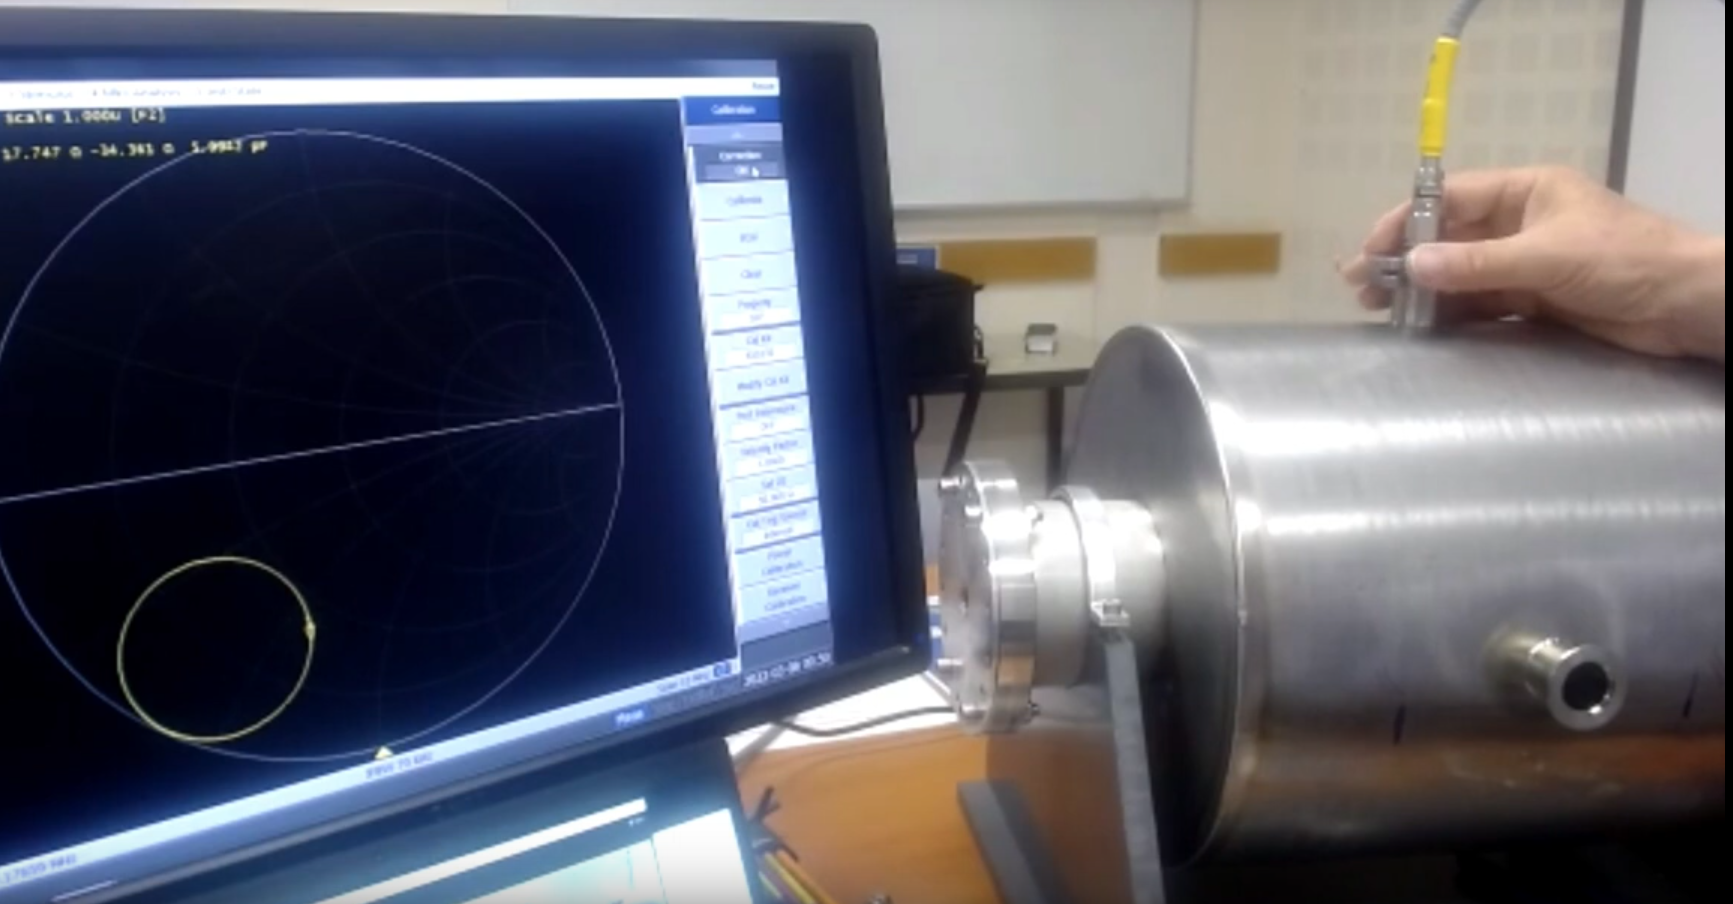
\includegraphics[height=0.15\textwidth]{img/cav_under.png}}\;
  \subfloat[Critically Coupled]{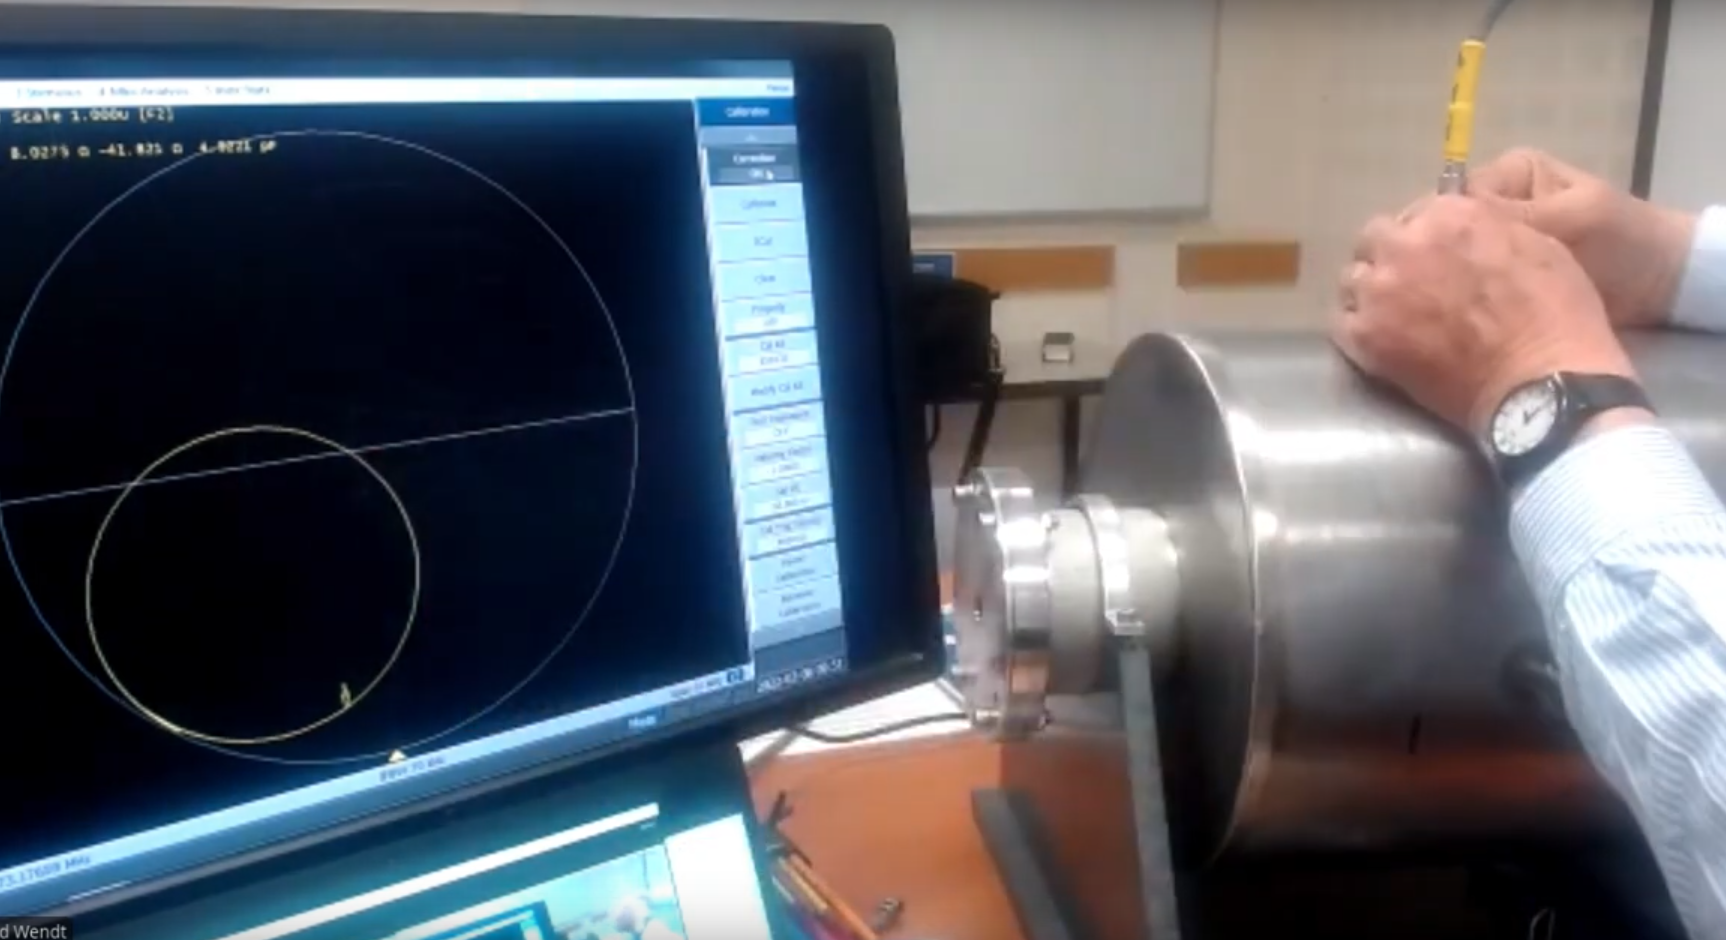
\includegraphics[height=0.15\textwidth]{img/cav_crit.png}}\;
  \subfloat[Over Coupled]{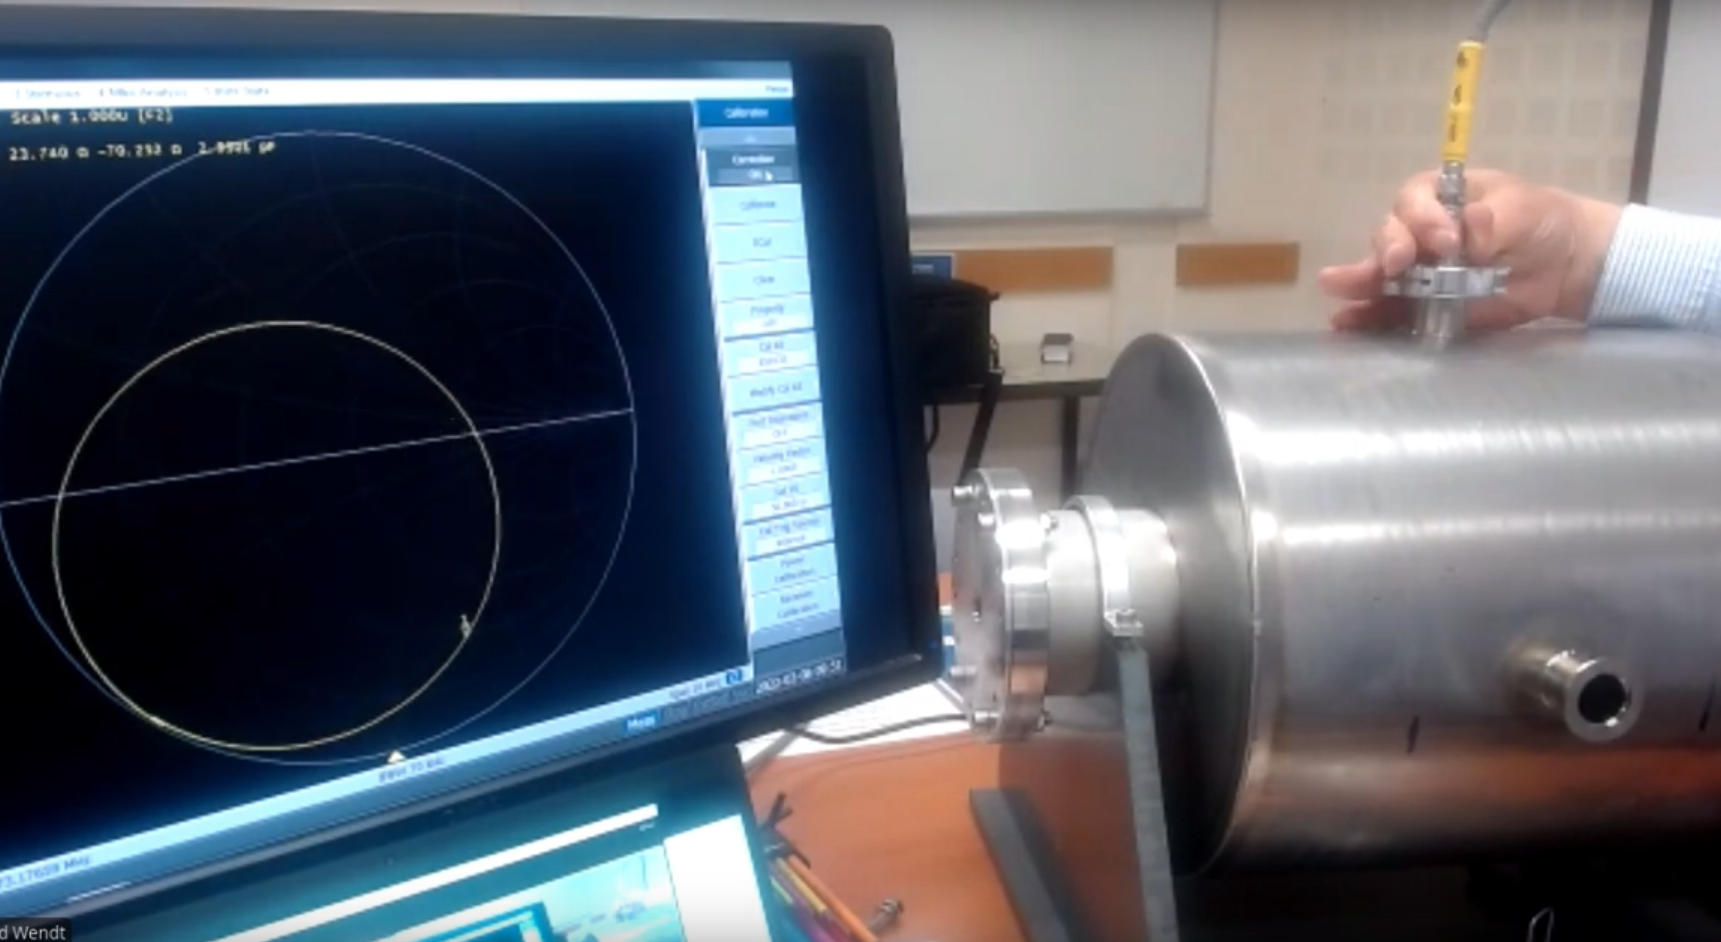
\includegraphics[height=0.15\textwidth]{img/cav_over.png}}
\end{figure}
\end{frame}

\section{Resume}
\begin{frame}[t,fragile]{Resume}
\begin{itemize}
\item Last session with Michele
\item We learned, that...
\item Whatever ...
\end{itemize}
\end{frame}

\end{document}
